\documentclass{beamer}

\usepackage{beamerthemesplit}
\usetheme{Singapore} %Copenhagen}
%\usecolortheme{whale}

%\usepackage[T2A]{fontenc}
%\usepackage[utf8]{inputenc}
%\usepackage[russian]{babel}

\usepackage[main=russian,english]{babel}   %% загружает пакет многоязыковой вёрстки
\usepackage{fontspec}      %% подготавливает загрузку шрифтов Open Type, True Type и др.
\defaultfontfeatures{Ligatures={TeX},Renderer=Basic}  %% свойства шрифтов по умолчанию
\setmainfont{Times New Roman} %% задаёт основной шрифт документа
%\usefonttheme{professionalfonts}% SOLUTION
\usefonttheme{serif}

\usepackage{hyperref}
\usepackage{textcomp}
\usepackage{amssymb,amsmath}
%\usepackage{animate}
%\usepackage{longtable}
\usepackage{xcolor}

%\usepackage{pgffor}
\usepackage{enumitem}
\usepackage[export]{adjustbox}

\newcounter{N}

%% Форматирование окружения itemize
%\usepackage{ragged2e}
%\let\olditem\item
%\renewcommand\item{\olditem\justifying}

\usepackage{ mathrsfs }
\newcommand{\Rho}{\mathscr{P}}

\renewcommand{\Re}{\operatorname{Re}}
\newcommand{\Sh}{\operatorname{Sh}}
\newcommand{\Eu}{\operatorname{Eu}}
\newcommand{\Fr}{\operatorname{Fr}}

%\DeclareMathOperator{\tg}{tg}
\DeclareMathOperator{\сtg}{сtg}


\newcommand{\argxi}{(\xi^1,\xi^2,\xi^3)}
\newcommand{\argx}{(x^1,x^2,x^3)}

\newcommand{\argxiv}{(\vec{\xi})}
\newcommand{\argxv}{(\vec{x})}


\newcommand{\argxbarn}{(\bar{x}^1,\bar{x}^2,\ldots, \bar{x}^n)}
\newcommand{\argxn}{(x^1, x^2,\ldots, x^n)}

\newcommand{\argtxi}{(t, \xi^1,\xi^2,\xi^3)}
\newcommand{\argtoxi}{(t_0, \xi^1,\xi^2,\xi^3)}

\newcommand{\argtxiv}{(t, \vec{\xi})}
\newcommand{\argtoxiv}{(t_0, \vec{\xi})}


\newcommand{\argtx}{(t, x^1,x^2,x^3)}
\newcommand{\argtox}{(t_0, x^1,x^2,x^3)}

\newcommand{\argtxv}{(t, \vec{x})}
\newcommand{\argtoxv}{(t_0, \vec{x})}


\newcommand{\pd}[2]{\frac{\partial #1}{\partial #2}}
\newcommand{\pdk}[2]{\frac{\partial^2 #1}{\partial #2^2}}

\newcommand{\od}[2]{\frac{d #1}{d #2}}
\newcommand{\odk}[3]{\frac{d^{#3} #1}{d #2^{#3}}}

\newcommand{\grad}{\operatorname{grad}}
\newcommand{\rot}{\operatorname{rot}}
\newcommand{\divo}{\operatorname{div}}

\title[]{Течения вязкой жидкости при малых числах Рейнольдса}

\author[]{ {\em Верещагин Антон Сергеевич}
\\
канд. физ.-мат. наук, старший преподаватель\\
\bigskip
Кафедра аэрофизики и газовой динамики ФФ НГУ}

\usebackgroundtemplate{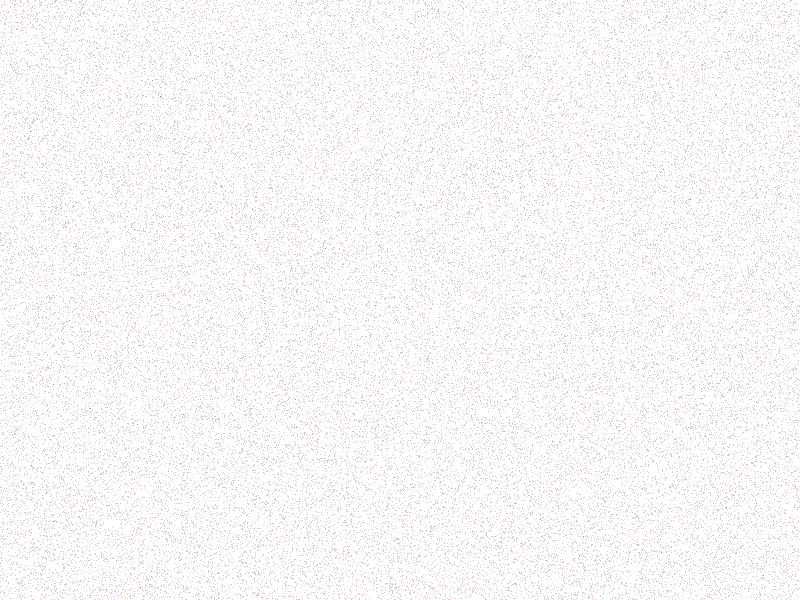
\includegraphics[width=\paperwidth]{../img/background.png}}

\begin{document}
	
\frame{\titlepage}


\frame{
	\frametitle{Аннотация}
	\parbox{\textwidth}{
	Задача обтекание сферы вязкой жидкостью. Модель Стокса. Решение задачи обтекания сферы в рамках модели Стокса. Сравнение со случаем обтекания идеальной жидкости. Сила Стокса. Применимость теории Стокса. Формулы Озеена, Озеена-Гольдстейна, Буссинеска.
	}
}

\frame{
	\frametitle{Обтекание сферы вязкой жидкостью }
	
	\centering
	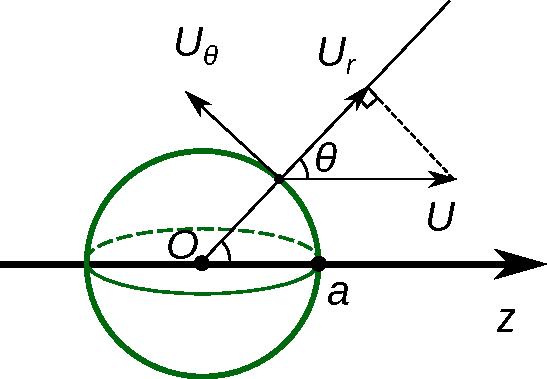
\includegraphics[width=0.5\textwidth]{../img/sphere.pdf}
	\begin{exampleblock}{Постановка задачи (\textit{G.G Stokes}, 1851)}
		\parbox{\textwidth}{
			Определить силу, действующую на сферу радиуса $a$, движущуюся со скоростью $U$ в потоке вязкой жидкости плотности $\rho$ и динамической вязкостью $\mu$, при малых числах Рейнольдса 
			\[
			\Re= \frac{2 a U \rho}{\mu} \ll 1.
			\]
		}
	\end{exampleblock}
	
}

\frame{
	\frametitle{Математическая постановка задачи}
	
	\begin{exampleblock}{}
		\parbox{\textwidth}{
			Задача обтекания движущейся сферы со скоростью $U$ эквивалентна задаче обтекания покоящейся сферы в начале координат с заданным значением скорости потока на бесконечности. Стационарное течение жидкости около сферы описывается уравнениями Навье-Стокса:
			\[
			\divo \vec{v} = 0,
			\]
			\[
			 (\nabla\cdot\vec{v})\vec{v} = -\frac{1}{\rho}\nabla p + \nu \Delta\vec{v}
			\]
			с граничным условием на сфере ($r=\sqrt{x^2+y^2+z^2}$)
			\[
			\vec{v}|_{r=a} = 0
			\]
			и на бесконечности при $r\to\infty$ 
			\[
			v_x\to 0,\quad
			v_y\to 0,\quad
			v_z\to U.
			\]
		}
	\end{exampleblock}
	
	
	
}

\frame{
	\frametitle{Уравнения Стокса}
	
	\begin{exampleblock}{Оценка слагаемых в уравнениях Навье-Стокса}
		\parbox{\textwidth}{
			
			\[
			\frac{\rho |(\nabla\cdot\vec{v})\vec{v}| }{\mu |\Delta\vec{v}|} \sim 
			\frac{\rho U^2}{2a} : \frac{\mu U }{(2a)^2} = \Re \ll 1.
			\]
		}
	\end{exampleblock}\pause

	\begin{exampleblock}{Модель Стокса для описания ползущих течений}
		\parbox{\textwidth}{
			Отбрасывая \alert{нелинейные инерционные члены} в уравнении импульса из модели Навье-Стокса, получим уравнения
			\[
			\divo \vec{v} = 0,\quad
			\nabla p = \mu \Delta\vec{v},
			\]
			которые будем решать в сферической системе координат. 
			
			\medskip
			Данная модель является \alert{линейной} относительно функций $p$ и $\vec{v}$ вида
			\[
				v_r = v_r(r,\theta),\quad
				v_\theta=v_\theta(r,\theta),\quad
				v_\lambda = 0,\quad
				p = p(r,\theta).
			\]
		}
	\end{exampleblock}
}

\frame{
	\frametitle{Задача обтекания сферы в постановке Стокса}
	
	\begin{exampleblock}{Основные уравнения}
		\parbox{\textwidth}{
		\[
		\pd{p}{r} = \mu\left(
		\pdk{v_r}{r}+\frac{1}{r^2}\pdk{v_r}{\theta}+\frac{2}{r}\pd{v_r}{r}+
		\frac{\ctg\theta}{r^2}\pd{v_r}{\theta} -\frac{2}{r^2} \pd{v_\theta}{\theta} -\frac{2}{r^2} \pd{v_\theta}{\theta}  - 
		\right.
		\]
		\[
		\left.
		-\frac{2 v_r}{r^2} - \frac{2\ctg \theta}{r^2}v_\theta
		\right),
		\]
		\[
		\frac{1}{r}\pd{p}{\theta} = \mu \left(
		\pdk{v_\theta}{r} + \frac{1}{r^2}\pdk{v_\theta}{\theta} + 
		\frac{2}{r}\pd{v_\theta}{r}+\frac{\ctg\theta}{r^2}\pd{v_\theta}{\theta} +
		\frac{2}{r^2}\pd{v_r}{\theta}-\frac{v_\theta}{r^2 \sin^2 \theta}
		\right),
		\]
		\[
		\pd{v_r}{r} + \frac{1}{r}\pd{v_\theta}{\theta} + \frac{2 v_r}{r} + \frac{v_\theta \ctg\theta}{r} = 0.
		\]	
		}
	\end{exampleblock}
	\vspace{-2mm}
	\begin{exampleblock}{Граничные условия}
		\parbox{\textwidth}{
		\[
		v_r(a,\theta) = 0,\quad
		v_\theta(a,\theta) = 0.
		\]
		\[
		v_r \overset{r \to \infty}{\to} U \cos\theta,\quad
		v_\theta \overset{r \to \infty}{\to} -U\sin\theta.
		\]	
		}
	\end{exampleblock}

	
	
}

\frame{
	\frametitle{ Решение }
	
	\begin{exampleblock}{Вид искомых функций}
		\parbox{\textwidth}{
		\[
			v_r(r,\theta) = f(r) \cos\theta,\quad
			v_\theta(r,\theta) = -g(r)\sin\theta,\quad
			p(r,\theta) = \mu h(r) \cos\theta.
		\]
		}
	\end{exampleblock}

	\begin{exampleblock}{Упрощение исходной системы}
		\parbox{\textwidth}{
			\[
			h' = f~''+\frac{2}{r}f~' - \frac{4(f-g)}{r^2},
			\]
			\[
			\frac{h}{r} = g'' +\frac{2}{r}g' + \frac{2(f-g)}{r^2},
			\]
			\[
			f~' + \frac{2(f-g)}{r} = 0.
			\]
			
		}
	\end{exampleblock}
	\begin{exampleblock}{Начальные условия}
		\parbox{\textwidth}{
			\[
			f(a) = 0,\quad
			g(a) = 0,\quad
			f(\infty) = U,\quad
			g(\infty) = U.
			\]
		}
	\end{exampleblock}
}

\frame{
	\frametitle{ Решение }
	
	\begin{exampleblock}{Метод исключения переменных }
		\parbox{\textwidth}{
			\[
			\left\{
			\begin{array}{l}
			g = \displaystyle f~'r/2+f,\\
			h = \displaystyle f~'''r^2/2+3rf~''+2f~',\\
			r^3 f~^{(4)} + 8 r^2 f~^{(3)} + 8rf~''-8f~'=0.
			\end{array}
			\right.
			\]
		}
	\end{exampleblock}\pause
	
	\begin{exampleblock}{Решение для уравнения типа Эйлера}
		\parbox{\textwidth}{
			Пусть $f = r^k$,
			тогда
			\[
			k(k-1)(k-2)(k-3) + 8k(k-1)(k-2) + 8k (k-1)-8k = 0.
			\]
			Решение
			\[
			k=0,\quad
			k=2,\quad
			k=-1,\quad
			k=-3.
			\]
		}
	\end{exampleblock}
	
}


\frame{
	\frametitle{ Решение }
	
	\begin{exampleblock}{Общий вид $f$, $g$, $h$}
		\parbox{\textwidth}{
			\[
			f = \frac{A}{r^3} + \frac{B}{r} + C + D r^2,
			\]
			\[
			g = -\frac{A}{2r^3}+\frac{B}{2r}+C + 2 D r^2,\quad
			h = \frac{B}{r^2} + 10 D r.
			\]
		}
	\end{exampleblock}

	\begin{exampleblock}{Уточнение констант из граничных условий}
		\parbox{\textwidth}{
			\[
			D = 0,\quad
			C = U,\quad
			B = -\frac{3}{2} U a,\quad
			A = \frac{1}{2}U a^3.
			\]
			
		}
	\end{exampleblock}
	
}

\frame{
	\frametitle{ Решение }
	
	\begin{exampleblock}{Скорость и давление}
		\parbox{\textwidth}{
		\begin{eqnarray*}
		v_r(r,\theta) & = & U \cos\theta 
		\left[
		1 - \frac{3}{2}\frac{a}{r} + \frac{1}{2}\frac{a^3}{r^3}
		\right],\\
		v_\theta(r,\theta) & = & -U \sin\theta 
		\left[
		1 - \frac{3}{4}\frac{a}{r} - \frac{1}{4}\frac{a^3}{r^3}
		\right],\\
		p(r,\theta) & = &  -\frac{3}{2}\mu\frac{Ua}{r^2}\cos\theta.
		\end{eqnarray*}
		}
	\end{exampleblock}\pause


}

\frame{
	\frametitle{ Сравнение с обтеканием сферы идеальной жидкостью }
	
	\begin{exampleblock}{Коэффициент давления}
		\parbox{\textwidth}{
				\[
			c_p = \frac{p-p_\infty}{\frac{1}{2}\rho U^2} = -\frac{3\mu}{\rho U a}\frac{\cos\theta}{(r/a)^2} =  -\frac{6}{\Re}\frac{\cos\theta}{(r/a)^2}.
			\]
		}
	\end{exampleblock}\pause

	

	\begin{enumerate}[label=(\arabic*)]
	\item Коэффициент давления является функцией числа Рейнольдса $\Re$ и угла $\theta$.\pause
	\item Распределение давления не симметрично относительно миделевой плоскости, так что главный вектор сил давления отличен от $0$ (парадокс Даламбера не имеет место).\pause
	\item Коэффициент давления в критических точках не равен единице; при $\theta=\pi/2$ давление равно давлению в невозмущенном потоке; максимальное разряжение достигается в задней критической точке.
	\end{enumerate}	

	
	
}


\frame{
	\frametitle{ Сила, действующая на тело со стороны  жидкости }
	\small
	\begin{exampleblock}{Компоненты тензора напряжений в сферической системе координат}
		\parbox{\textwidth}{

			\[
			\sigma_{rr} = -p+2\mu\pd{v_r}{r},\quad
			\sigma_{r\theta} = \mu\left(\frac{1}{r}\pd{v_r}{\theta}+\pd{v_\theta}{r}-\frac{v\theta}{r}\right),
			\]
			\[
			\sigma_{\theta\theta} = -p + 2\mu\left(\frac{1}{r}\pd{v_\theta}{\theta}+\frac{v_r}{r}\right),\quad
			%	\]
			%	\[
			\sigma_{\theta\lambda} = \mu\left(
			\frac{1}{r\sin\theta}\pd{v_\theta}{\lambda}+\frac{1}{r}\pd{v_\lambda}{\theta}-
			\frac{v_\lambda\ctg\theta}{r}
			\right),
			\]
			\[
			\sigma_{\lambda\lambda} = -p + 2\mu\left(
			\frac{1}{r\sin\theta}\pd{v_\lambda}{\lambda}+\frac{v_r}{r}+
			\frac{v_\theta\ctg\theta}{r}
			\right),
			\]
			\[
			\sigma_{\lambda r} = \mu\left(
			\pd{v_r}{r} + \frac{1}{r\sin\theta}\pd{v_r}{\lambda}-\frac{v_\lambda}{r}
			\right).
			\]
		}
	\end{exampleblock}

	\begin{exampleblock}{Сила}
		\parbox{\textwidth}{
		\[
		\vec{F} = \int_S \vec{n}\cdot\sigma dS,
		\]
		где $S$ -- поверхность тела, $\vec{n}$ -- вектор внешней единичной нормали, направленный в жидкость.
		}
	\end{exampleblock}
	

	
}



\frame{
	\frametitle{ Сила Стокса }
	
	\begin{exampleblock}{Компоненты тензора напряжений на поверхности сферы}
		\parbox{\textwidth}{
			\[
			\sigma_{rr}|_{r=a} = \left( -p + 2 \mu \pd{v_r}{r}\right)_{r=a} = \frac{3}{2}\mu\frac{Ua}{r^2}\cos\theta,
			\]		
			\[
			\sigma_{r\theta}|_{r=a} = \mu\left(\frac{1}{r}\pd{v_r}{\theta}+\pd{v_\theta}{r} -\frac{v_\theta}{r} \right)_{r=a}=-\frac{3\mu U}{2a}\sin\theta.
			\]	
		}
	\end{exampleblock}\pause
	
	\begin{exampleblock}{Сила, действующая на сферу}
		\parbox{\textwidth}{
			\[
			W = \int\limits_S (\sigma_{rr}\cos\theta - \sigma_{r\theta}\sin\theta) dS = 
			\int\limits_0^\pi (\sigma_{rr}\cos\theta - \sigma_{r\theta}\sin\theta) 2 \pi a^2 \sin\theta d\theta = 
			\]
			\[
			=
			3\pi\mu U a \int\limits_0^\pi \sin\theta d\theta =
			6\pi\mu U a.
			\]
			
		}
	\end{exampleblock}

}

\frame{
	\frametitle{ Границы применимости формулы Стокса }
	
	\centering
	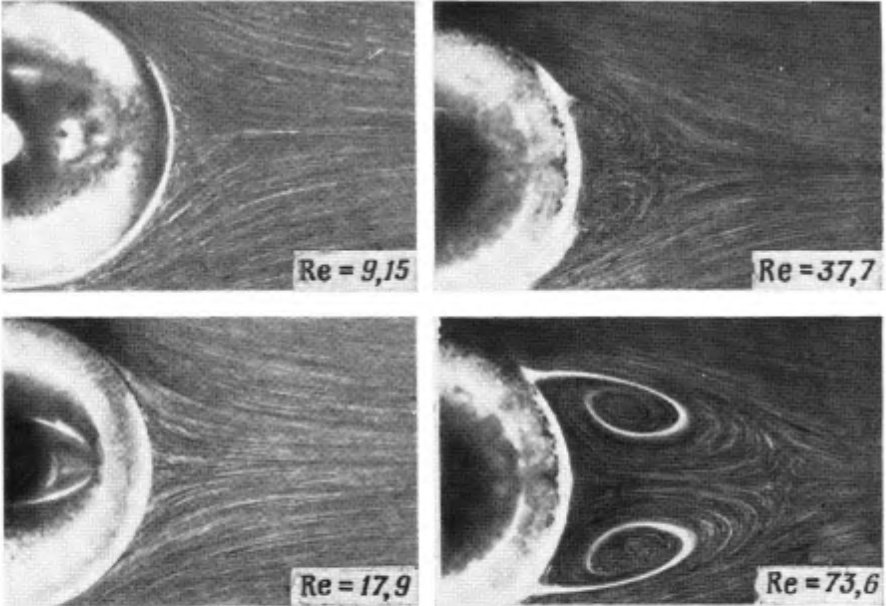
\includegraphics[width=0.9\textwidth]{../img/flow_sphere_1.png}\\
	
	Линии тока в осевой плоскости установившегося течения около сферы радиуса $a$ (Танеда, 1956б).
	
	
}


\frame{
	\frametitle{ Границы применимости формулы Стокса }
	
	\centering
	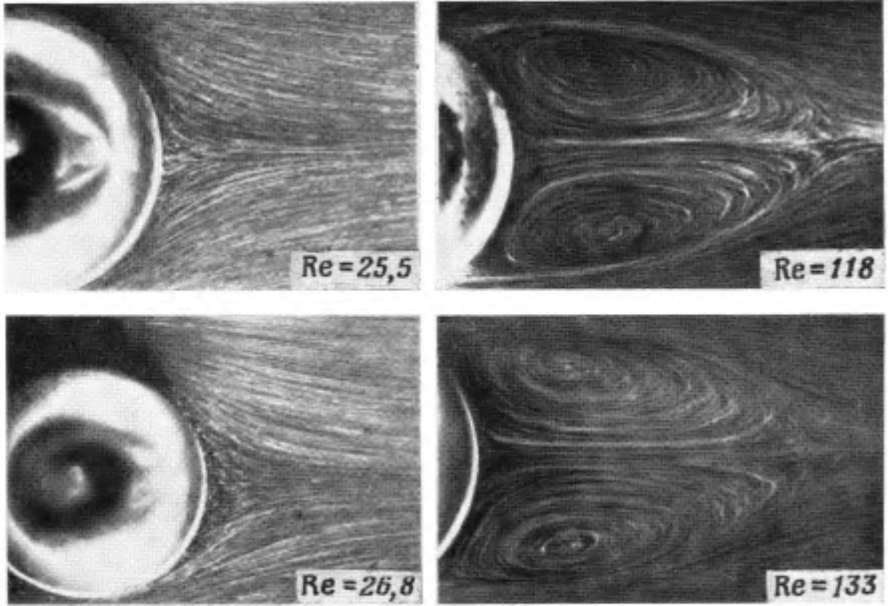
\includegraphics[width=0.9\textwidth]{../img/flow_sphere_2.png}\\
	
	Линии тока в осевой плоскости установившегося течения около сферы радиуса $a$ (Танеда, 1956б).
	
	
}

\frame{
	\frametitle{Коэффициент сопротивления}
	
	\begin{exampleblock}{Коэффициент сопротивления для решения Стокса}
		\parbox{\textwidth}{
		
		\medskip
		\[
			c_z = \frac{W}{\frac{1}{2}\rho U^2 \pi a^2} = 
			\frac{6\pi \mu a U}{\frac{1}{2}\rho U^2 \pi a^2} = \frac{24}{\Re}.
		\]
%		\[
%			\Re = \displaystyle\frac{\rho U d}{\mu} = \frac{U d}{\nu},\quad
%			d=2a.
%		\]
		}
	\end{exampleblock}\pause

	\begin{exampleblock}{Теория Озеена и Озеена-Гольдстейна}
		\parbox{\textwidth}{
			\[
			c_z = \frac{24}{\Re}\left(
			1 + \frac{3}{16}\Re-\frac{19}{1280}\Re^2+\ldots			
			\right).
			\]
			Если сохранить только первый член, то будет формула Стокса, первые два -- формула Озеена и т.д. 
			
			\medskip
			Формула Озеена получается при лианеризации конвективного слагаемого в уравнениях Навье-Стокса по формуле
			\[
			(\vec{v}\cdot\nabla)\vec{v} \approx (\vec{U} \cdot\nabla)\vec{v}.
			\]
		}
	\end{exampleblock}

}

\frame{
	\frametitle{ Сравнение теорий }
	\centering
	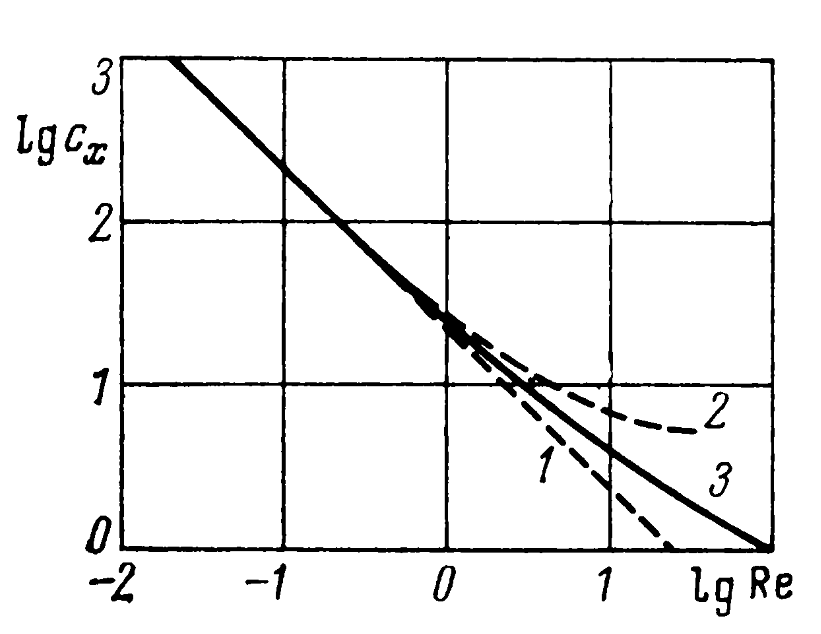
\includegraphics[width=0.8\textwidth]{../img/cx.png}\\
	
	Зависимость коэффициента сопротивления сферы от числа Рейнольдса (1 -- Стокс, 2 -- Озеен, 3 -- эксперимент)
}


\frame{
	\frametitle{ Другие решения уравнений Стокса }
	
	\begin{exampleblock}{Постановка задачи}
		\parbox{\textwidth}{
			Определить силу сопротивления сферы радиуса $a$ потоку вязкой несжимаемой жидкости плотности $\rho$ и вязкости $\mu$, движущемуся  поступательно с заданной переменной скоростью $\vec{U}(t)$ ($\vec{U}(0)=0$).
		}
	\end{exampleblock}\pause
	
	\begin{exampleblock}{Формула Буссинеска}
		\parbox{\textwidth}{
			\[
			\vec{W} = -\underbrace{6\pi\mu a \vec{U}(t)}_{\text{Стокс}}  \underbrace{-\frac{2}{3}\pi\rho a^3\vec{U}'(t)}_{\text{присоединенная масса}} -
			\underbrace{6\pi\mu a^2 \frac{1}{\sqrt{\pi\nu}}
			\int\limits_0^t \frac{\vec{U}'(\tau) d\tau}{\sqrt{t-\tau}}}_{\text{Бассе}}.
			\]\pause
			
			\vspace{-5mm}			
			Сила для импульсно приведённого из состояния покоя в движения шара до скорости $U_0$
			\[
			W = 6\pi\mu a U_0 \left(1 + \sqrt{\frac{a^2}{\pi\nu t}}\right).
			\]
		}
	\end{exampleblock}
	
}


\frame{
	\frametitle{ Литература }
	\begin{itemize}[partopsep=1pt,label=\textbullet]
		\item {\em Кочин~Н.~Е., Кибель~И.~А., Розе~Н.~В.} Теоретическая гидромеханика. М.:Гос. издат. физ.-мат. лит., 1963.
		
		\item 
		{\em Лойцянский~Л.~Г.} Механика жидкости газа и плазмы: Учеб. для вузов. --- 7-е изд., испр. -- М.:Дрофа, 2003
		
		\item {\em Бэтчелор Дж.} Введение в динамику жидкости. --- М.: Мир, 1973.
		
		\item {\em Ландау~Л.~Д., Лифшиц~Е.~М.} Теоретическая физика: Учебное пособие. В 10 т. Т. VI. Гидродинамика. -- 3-е изд., перераб. --- М.: Наука. Гл. ред. физ-мат. лит., 1986.
		
		
	\end{itemize}
}



\end{document}